\chapter{\MakeUppercase{Introducción}}
\thispagestyle{mainmatterstyle} % Cambia el estilo para que este numerado en la esquina superior derecha. Esta presente en todos los chapter

\section{Problemática} \label{problematic}

Entre enero y mayo de 2022, las exportaciones de camisas, pantalones y camisetas en Perú experimentaron incrementos notables, con crecimientos del 57\%, 49\% y 31\% en valor, respectivamente. Hasta mayo de 2022, las exportaciones de confecciones alcanzaron los 759 millones de dólares americanos, marcando un aumento del 36\% en comparación con el año anterior \cite{LaCamara2022}. Estas estadísticas demuestran un crecimiento significativo en la exportación de prendas de vestir peruanas, por lo cual, es importante mantener altos estándares de calidad para satisfacer las expectativas de los mercados internacionales.

\begin{figure}[H]
	\centering
	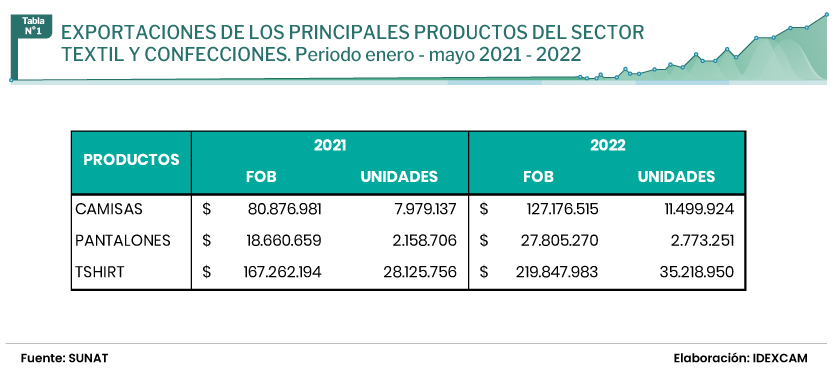
\includegraphics[width=0.9\textwidth]{exportaciones.jpg}
	\caption[Exportaciones peruanas de textiles: aumento en FOB y unidades, 2021 vs 2022.]{Exportaciones peruanas de textiles: aumento en FOB y unidades, 2021 vs 2022. Fuente \cite{LaCamara2022}.}
\end{figure}

El control de calidad en la industria textil es esencial para asegurar que las prendas no solo cumplan con los estándares de calidad establecidos, sino también que ofrezcan seguridad y durabilidad. Este proceso minucioso abarca diversas etapas, incluyendo la inspección de tejidos, la graduación de patrones, el corte, la costura, el acabado y finalmente, el empaquetado. Todo ello con el objetivo de garantizar que el producto final cumpla con las expectativas de los clientes. Entre los defectos más comunes que se identifican durante estas etapas se encuentran las variaciones de color, manchas, agujeros, puntadas rotas, costuras desalineadas, hilos sueltos, así como medidas incorrectas y tallas inconsistentes, tanto en los tejidos como en la construcción de las prendas \cite{TetraInspection2024}. 

El enfoque tradicional de control de calidad, que se centra principalmente en inspecciones al final del proceso y en la implementación de correcciones a posterior, resulta en elevados costos debido a desechos y reparaciones. Este enfoque repercute negativamente en la competitividad y sostenibilidad de las empresas. Un estudio realizado por \cite{BonillaPastor2015} sobre la gestión de calidad en micro y pequeñas empresas (Mypes) del sector textil en Perú, destaca las graves consecuencias económicas y ambientales que surgen de una gestión de calidad ineficaz. Desde el punto de vista económico, los residuos y desperdicios producidos por procesos ineficientes constituyen un gasto promedio del 7.4\% en relación con el costo total de producción, lo cual impacta directamente en la competitividad y la rentabilidad de las empresas.

El control de calidad manual, como se observa en la Figura \ref{fig:insp_manual}, es ampliamente utilizada en procesos de producción debido a su relativa facilidad y la no necesidad de equipos técnicos especializados. Sin embargo, enfrenta desafíos significativos debido a factores humanos como los que se detallan en la Tabla \ref{tab:eficiencia_inspección}. Dichos factores inciden directamente en la efectividad del control de calidad manual, elevando potencialmente la incidencia de errores en la evaluación de la calidad. Investigaciones referenciadas en el estudio de \cite{KujawinskaVogt2015} revelan que, en tareas de inspección simples, la tasa de error puede fluctuar entre un 3\% y un 30\%, dependiendo de la índole de la tarea y las condiciones en que se efectúa la inspección.

\begin{figure}[H]
	\centering
	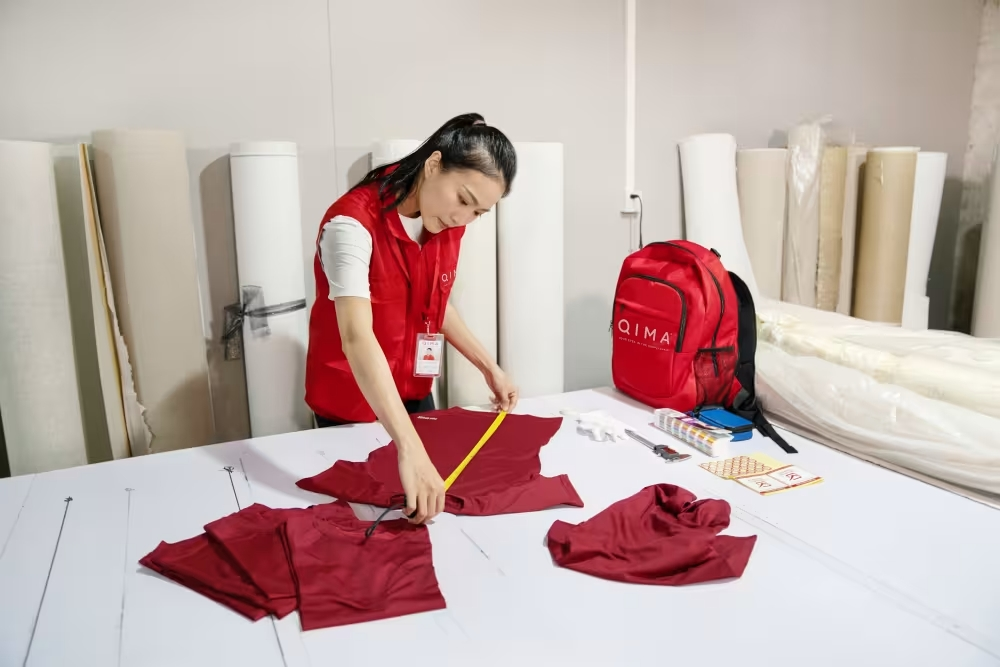
\includegraphics[width=0.65\textwidth]{insp_manual.jpg}
	\caption[Inspección manual de prendas de vestir.]{Inspección manual de prendas de vestir. Fuente \cite{qimaProcedimientosInspeccin}.}
	\label{fig:insp_manual}
\end{figure}

La integración de la Inteligencia Artificial (IA) en el control de calidad de la industria textil y de la moda ha introducido métodos avanzados para la inspección de calidad, desde la producción hasta la revisión final de las prendas. Esta innovación mejora significativamente la eficiencia y precisión, minimizando los errores humanos y los costos de producción, mientras asegura la adherencia a estándares de calidad elevados \cite{TextileLearner}. La Tabla \ref{tab:visual_vs_automated} resume la comparación entre inspección visual humana y la inspección automatizada. Estas limitaciones subrayan la necesidad de un proceso de inspección más automatizado y preciso para reducir errores y mejorar la eficiencia \cite{Islam2006ASuitable}.

\begin{table}[H]
	\centering
	\caption[Factores que afectan la eficiencia de la inspección visual.]{Factores que afectan la eficiencia de la inspección visual. Fuente \cite{KujawinskaVogt2015}.}
	\begin{tabular}{|p{10em}|p{20em}|}
		\hline
		\textbf{Factors} & \textbf{Examples}\\
		\hline
		Technical & {Type of defects; Defect visibility; Quality level; Standards (tests); Control automation;  Other}\\
		\hline
		Psychophysical & Age;  Sex;  Observation  skills;  Experience;  Temperament;  Creativity;  Other\\
		\hline
		Organizational & Training;  Scope  of  decision  making; Feedback;  Precise  instructions;  Other\\
		\hline
		Workplace environment & {Light; Noise; Temperature; Work time; Workstation organization; Other}\\
		\hline
		Social & {Team communication;  Pressure;  Isolation; Other}\\
		\hline
	\end{tabular}%
	\label{tab:eficiencia_inspección}%
\end{table}%

La automatización en la detección de defectos mediante visión artificial es crucial en manufactura, mejorando la consistencia y reduciendo errores humanos. La inspección óptica automatizada, impulsada por aprendizaje profundo y machine learning, supera los métodos manuales, ofreciendo eficiencia y precisión. Esto facilita la identificación rápida y confiable de defectos, elevando la calidad del producto y disminuyendo costos y tiempos de producción. La utilización de redes neuronales convolucionales para la extracción de características mejora la adaptabilidad y eficiencia de la inspección, siendo clave para el avance en manufactura. \cite{SanchezRomero2023}.

\begin{table}[H]
	\centering
	\caption[Inspección visual versus inspección automatizada.]{Inspección visual versus inspección automatizada. Fuente \cite{Islam2006ASuitable}.}
	\begin{tabular}{|p{13em}|c|c|}
		\hline
		\textbf{Inspection Type} & {\textbf{Visual}} & \textbf{Automated} \bigstrut\\
		\hline
		Fabric Types & 100\% & \multicolumn{1}{c|}{70\%} \bigstrut\\
		\hline
		Defect Detection Rate & 70\%  & 80\%+ \bigstrut\\
		\hline
		Reproducibility & 50\%  & 90\%+ \bigstrut\\
		\hline
		Objective Defect Judgment & 50\%  & {100\%} \bigstrut\\
		\hline
		Statistics Ability & 0\%   & 95\%+ \bigstrut\\
		\hline
		Inspection Speed & {30 m/min} & {120 m/min} \bigstrut\\
		\hline
		Response Type & 50\%  & {80\%} \bigstrut\\
		\hline
		Information Content & 50\%  & 90\%+ \bigstrut\\
		\hline
		Information Exchange & 20\%  & 90\%+ \bigstrut\\
		\hline
	\end{tabular}%
	\label{tab:visual_vs_automated}%
\end{table}%

\section{Propuesta de Solución}

Para hacer frente a la problemática expuesta en el Sección \ref{problematic}, el presente trabajo de investigación tiene como propuesta solución un sistema integral de control de calidad para la industria de la confección, diseñado para asegurar la ausencia de defectos visuales, la precisión en las tallas y la eliminación de elementos metálicos peligrosos como agujas en las prendas. El objetivo principal es lograr que el sistema opere de manera autónoma. En otras palabras, se busca reducir la intervención humana al mínimo necesario. Esta intervención se limita a tareas como la inserción de la prenda a verificar en el sistema, el ingreso de señales de control y la posterior retirada de la prenda ya evaluada. Por otro lado, el sistema limitará su evaluación exclusivamente a prendas de punto, es decir, aquellas confeccionadas mediante el tejido de hilo o lana utilizando agujas o maquinaria especializada. Este sistema avanzado busca mejorar la eficiencia en la inspección de calidad ya que será capaz de identificar y clasificar automáticamente defectos, asegurando que las prendas cumplan con los más altos estándares. Con un enfoque en la automatización y la tecnología, este sistema no solo garantiza una verificación eficaz de la calidad de las prendas, sino también optimiza los procesos de producción, mejorando la productividad de la industria textil.

\section{Objetivos}

El proyecto presenta un objetivo general del cual surgen \ref{lst:objetivos_especificos} objetivos específicos para lograr el cumplimiento del objetivo general.

\subsection{Objetivo General}

Desarrollar un sistema integrado para el control de calidad de prendas de vestir para inspeccionar cada prenda de manera individual, asegurando su conformidad con los estándares de calidad establecidos en la ficha técnica de la prenda, tales como la ausencia de defectos visibles, la precisión en las medidas de talla y la ausencia de elementos metálicos extraños.

\subsection{Objetivos Específicos}

\begin{enumerate}
	\setlength\itemsep{-0.5em}
	\item Realizar una revisión bibliográfica (estado del arte) que permita definir los requerimientos del diseño del sistema y todo lo concerniente al diseño conceptual.
	
	\item Definir las exigencias específicas que debe cumplir el sistema para lograr el objetivo principal.
	
	\item Diseñar un subsistema mecánico que permita transportar las prendas de vestir a través de los distintos módulos del sistema.
	
	\item Diseñar un subsistema de inspección por procesamiento de imágenes para realizar la medición de la talla de las prendas y realizar la verificación según la ficha técnica de la prenda.
	
	\item Diseñar un subsistema de detección de metales que examine cada prenda para identificar y alertar sobre la presencia de agujas, alfileres o cualquier otro elemento metálico extraño, garantizando así la seguridad del producto final.
	
	\item Desarrollar una interfaz intuitiva para mostrar resultados de detección de calidad de prendas, incluyendo visualización de defectos, mediciones de tallas e identificación de metales
	
	\item Estimar un costo de fabricación de un prototipo a partir de los componentes seleccionados.
	
	\label{lst:objetivos_especificos}
\end{enumerate}

